
\section{Cold Spray}\label{sec:cold-spray}
Most engineering alloys, including stainless steel, aluminium and titanium, will undergo solid-state bonding when two atomically flat and clean surfaces are brought into contact, particularly in vacuum environments, where surface contamination is minimal~\cite{merstallinger2009coldwelding}. This phenomenon is known as cold welding and occurs because the surface energy of the separated metal interfaces is higher than that of the bonded state, making direct bonding thermodynamically favourable~\cite{WagleBaker2015}. 

Designs typically aim to prevent this for space applications, but it is the core mechanism that underpins CSAM.\@ By accelerating metal powder particles to supersonic velocities and then impacting them onto the substrate, the particles cold weld to the surface, forming a deposit. As seen in \autoref{fig:cs}, the particles plastically deform on impact, causing the disruption and removal of the oxide layer, and exposing clean metal surfaces. 
\begin{figure}[htbp]
    \centering
    
    \begin{minipage}{0.45\textwidth}
        \centering
        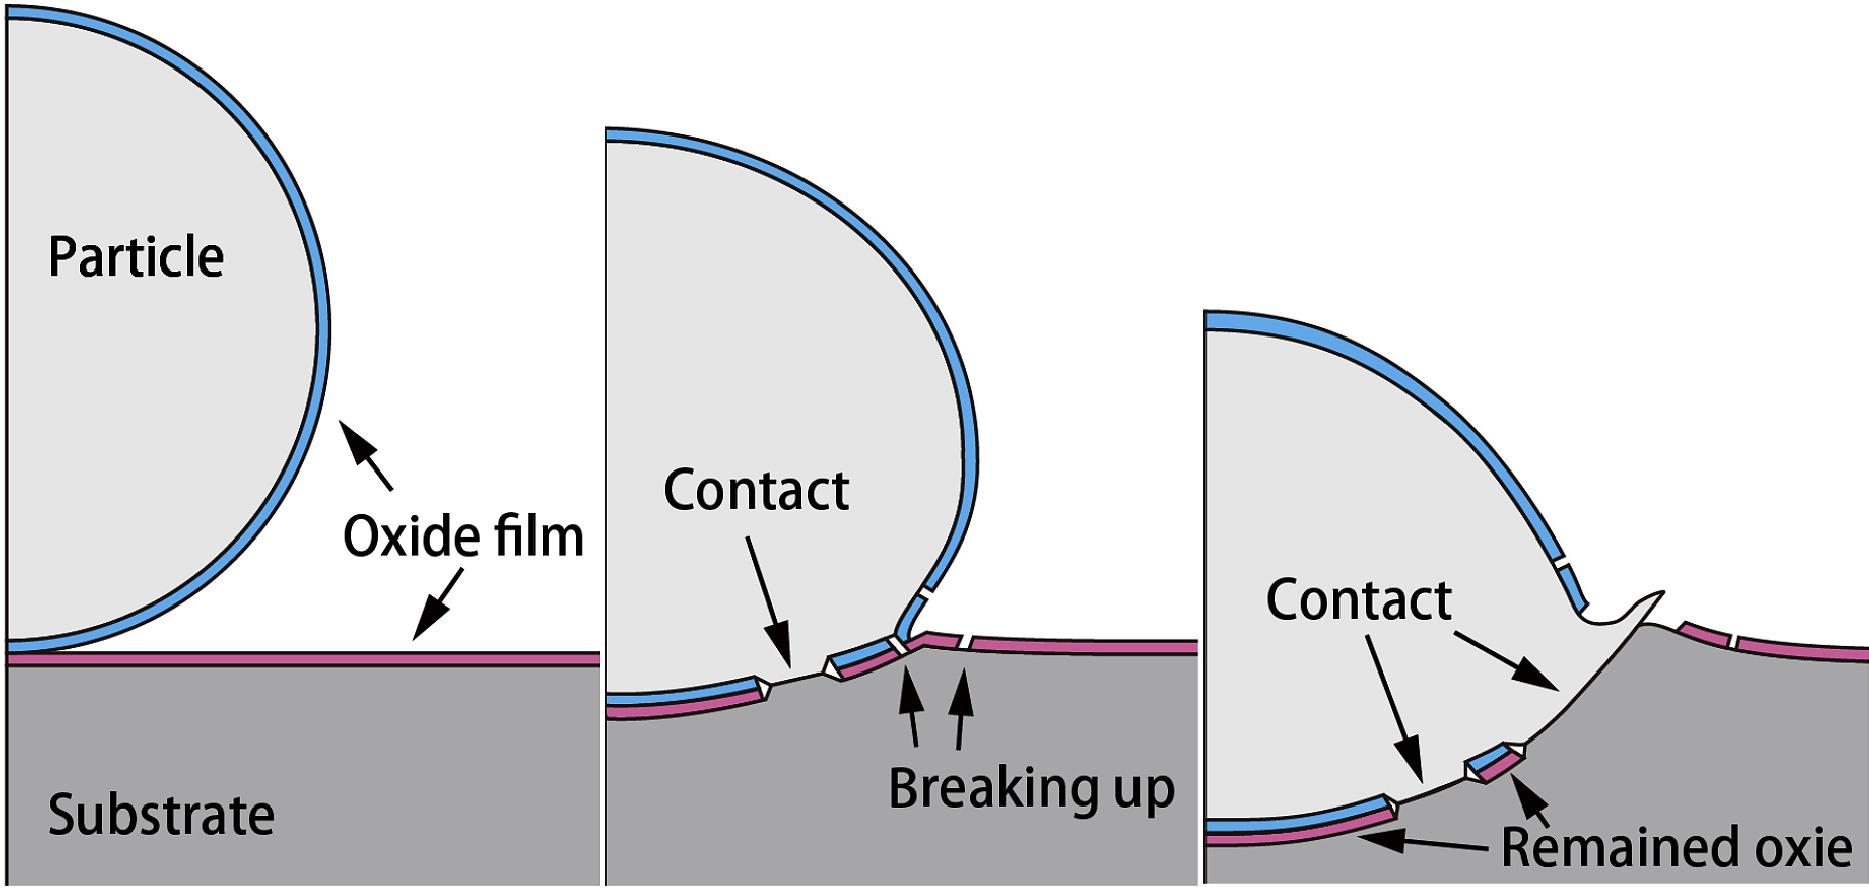
\includegraphics[width=\textwidth]{../report_assets/cs_bonding.png}
        \caption{Deformation and Bonding~\cite{ZHANG2024137157}}\label{fig:cs}
    \end{minipage}
    \hfill
    \begin{minipage}{0.45\textwidth}
        \centering
        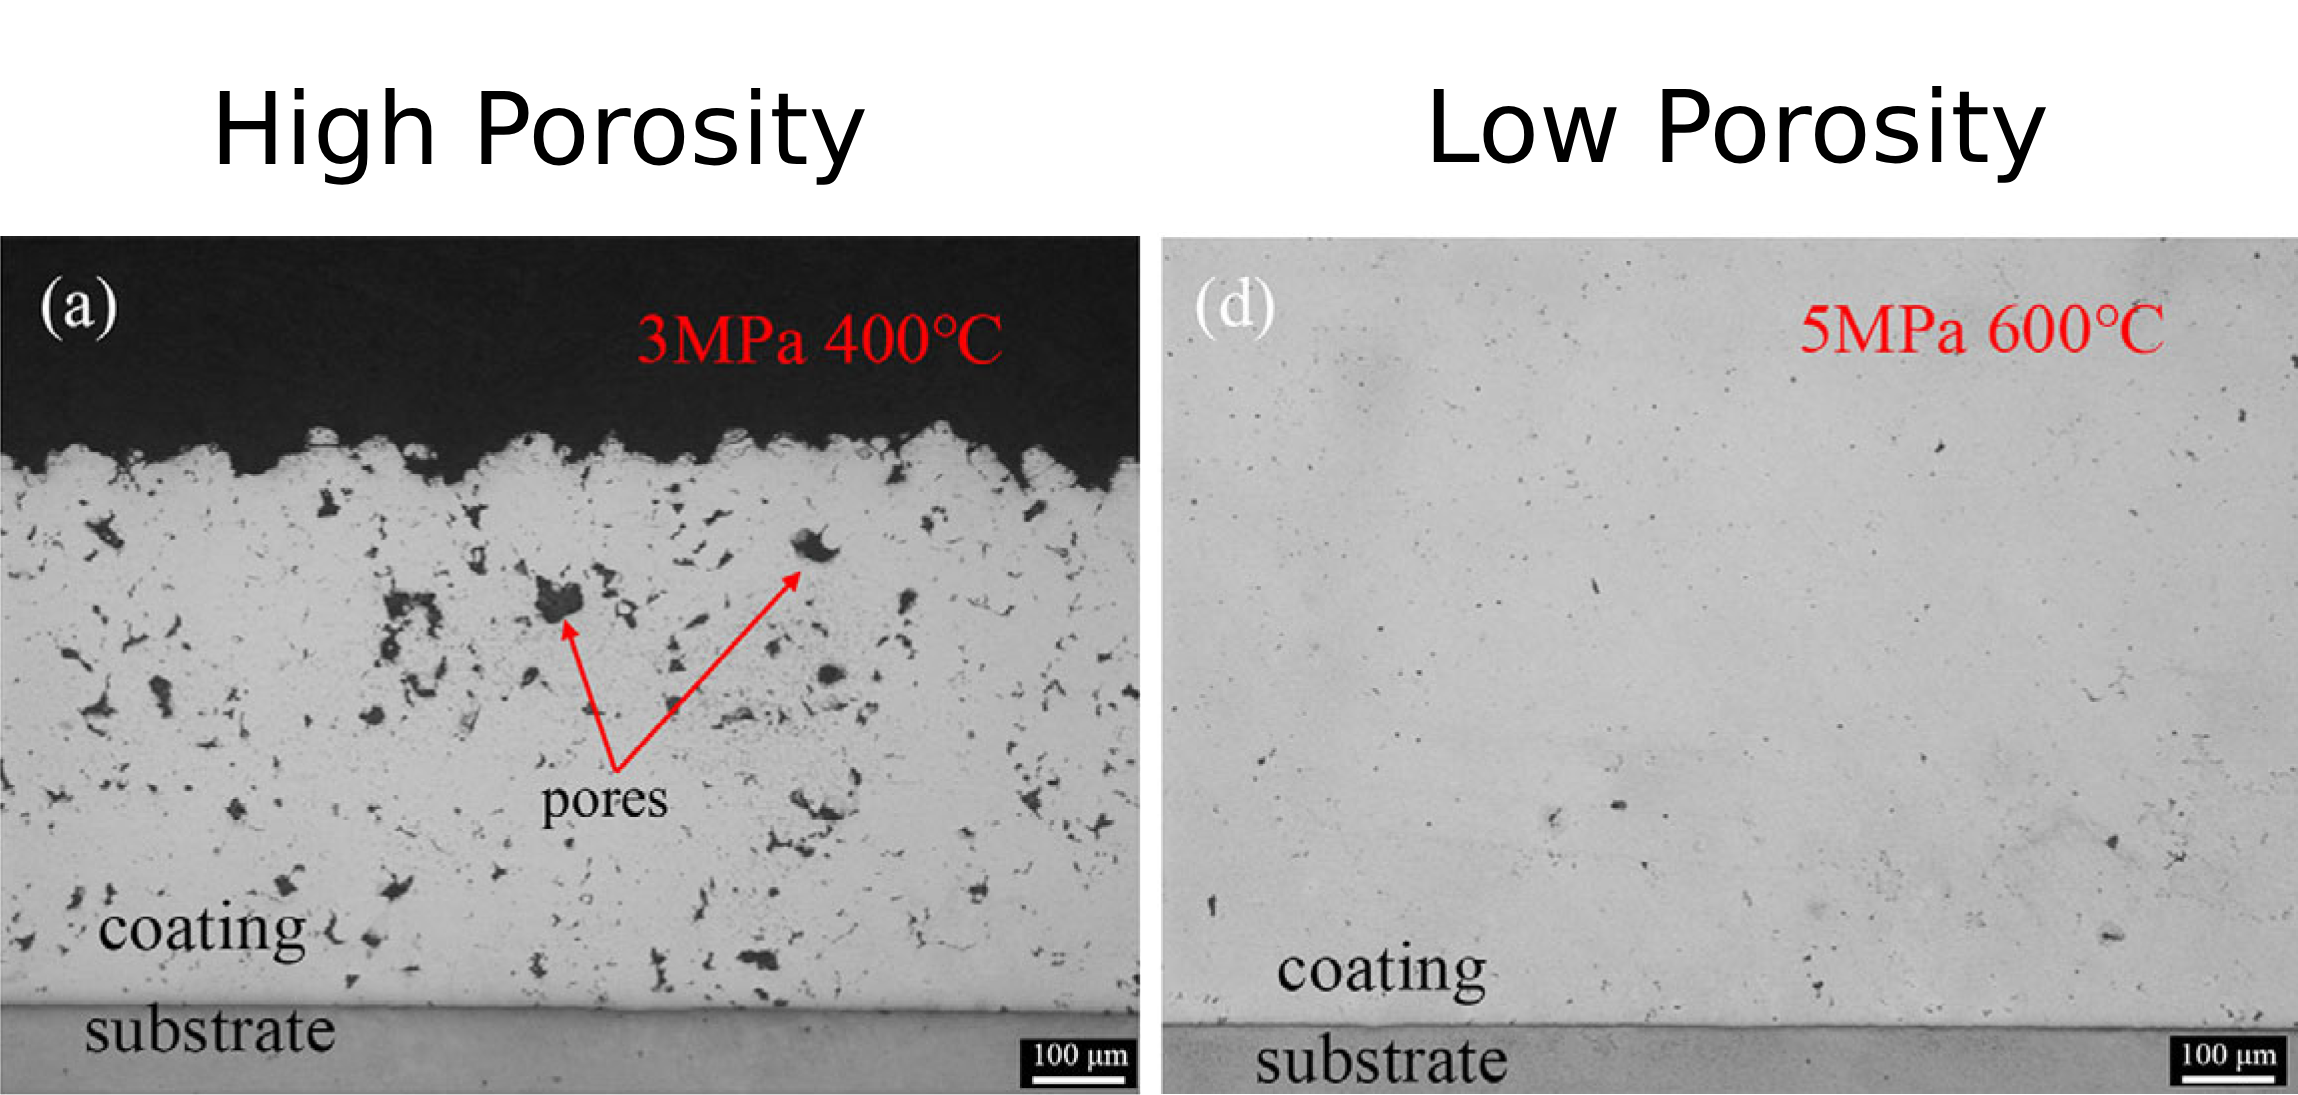
\includegraphics[width=\textwidth]{../report_assets/cs_porosity (1).png}
        \caption{Test Samples of CSAM~\cite{coatings13040738}}\label{fig:cs-porosity}
    \end{minipage}
    
\end{figure}
The removal of the oxide layer is thought to result from adiabatic shear instability at the particle-substrate interface~\cite{assadi2016cold}; however, the precise mechanisms remain a topic of ongoing research and debate within the field~\cite{HASSANIGANGARAJ2018430}.

A unique advantage of CSAM is that it is a solid-state manufacturing process. Because the material never transitions through a liquid phase, thermal input remains low, preserving the original microstructure of both the powder and the underlying substrate. This minimises issues such as residual thermal stresses, material oxidation and chemical composition inhomogeneity~\cite{ma16072765}. While solid-state manufacturing also tends to be better at reducing porosity, \autoref{fig:cs-porosity} shows that this can still be a problem depending on the parameters of the system. 

Arguably the most important parameter is the velocity of the particle impacting the surface. If this velocity is too low then bonding does not occur and if it is too high the powder roughens or erodes the substrate~\cite{Guo2022}. This velocity is dependent on the choice, pressure and temperature of accelerant gas and properties of the powder such as mass flow rate, size, shape and hardness. All of these must be carefully chosen or controlled to produce high-quality deposits.


\section{Fluidised Powder Bed Phenomenon}\label{sec:background-powder-beds}
Given that fluidisation underlies the design architecture presented later, the physics behind a generic fluidised powder bed are outlined in this section. The powder in these systems exhibits distinctive fluid-mechanical behaviour once a sufficient gas flow is passed upward through the granular solid~\cite{KuniiLevenspiel1977}. As shown in \autoref{fig:fluidisation}, as the gas velocity increases from zero, the powder initially remains fixed, with the gas passing through void spaces, known as a fixed bed regime. At a critical threshold, the minimum fluidisation velocity, the drag force exerted by the gas equals the effective weight of the particles, causing the bed to loosen and particles to become suspended.
\begin{figure}[htbp]
    \centering
    
    \begin{minipage}{0.45\textwidth}
        \centering
        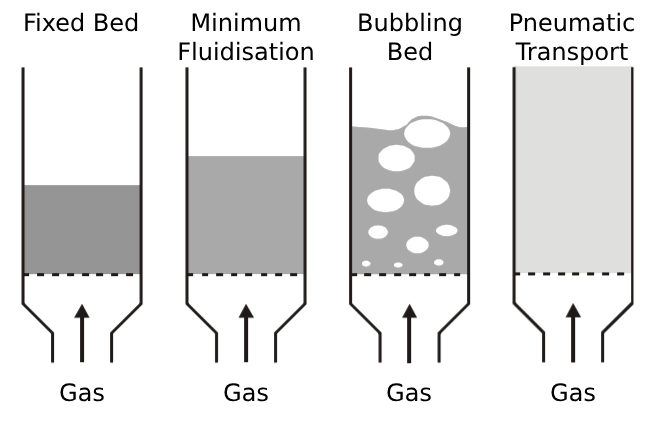
\includegraphics[width=\textwidth]{../report_assets/fluidisation_phases_diagram.png}
        \caption{Different Phases of Fluidisation~\cite{klaren2021fluidization}}
    \end{minipage}
    
\end{figure}\label{fig:fluidisation}
At this threshold, the pressure drop across the bed reaches a plateau, approximately matching the weight of the solid particles per unit area. The powder itself begins to swell in volume, a phenomenon known as bed expansion. This expansion corresponds to an increase in average porosity as particles are pushed further apart in the fluid-like suspension. With further increases in gas flow, the fluidised bed exhibits bubbling behaviour. In gas-fluidised systems at ambient pressure, any gas in excess of that required to just fluidise the bed passes through in the form of buoyant gas voids or bubbles~\cite{SHENG2022137168}.

At the particle scale, motion results from the interplay of buoyancy, drag, and either cohesive or gravitational forces, depending on the particle size. For smaller particles with a diameter of $20\,\mu\mathrm{m}$, numerical studies have shown that cohesion dominates, while particles of $75\,\mu\mathrm{m}$ are more influenced by gravity~\cite{SUN201785}. This means that the equilibrium for heavier particles may break down in microgravity, making space-based applications particularly challenging to predict or analyse. While research exists on particle dynamics under microgravity conditions, no literature was found specifically on the behaviour of fluidised powder beds or how to model them in a low gravity environment. Therefore, the effects of microgravity on the fluidisation physics are considered out of scope for this project and have been disregarded, with the assumption that fluidisation will still occur due to cohesion.


\section{Fluidised Powder Feed System Design Evolution}\label{sec:fluidised-powder-feed-systems}
The final architecture chosen in \autoref{sec:system_architecture} draws heavily from research into metallic powder-fed engines. As both systems have strict requirements for mass flow rate control and miniaturisation, this analysis can be used to inform a more elegant design. These systems have undergone multiple revisions to optimise performance, and this timeline is outlined to better explain the design's behaviour.

A commonly cited first implementation of a fluidising powder feed system consists of a cylindrical tank with a piston used to constrain the powder to the outlet~\cite{LI2021712}. As this paper is no longer in the public domain, exact parameters are unknown, but developments from this design can be grouped into three phases.

The first of these improvements is the use of a gas-actuated piston instead of one driven by a motor~\cite{TANG2023118406}. Examples of both approaches are shown in \autoref{fig:actuation-piston}. The additional mass of an electric motor, along with the electrical systems to support it, can be avoided by rerouting the high-pressure line present near the tank.
\begin{figure}[htbp]
    \centering
    
    \begin{minipage}{0.35\textwidth}
        \centering
        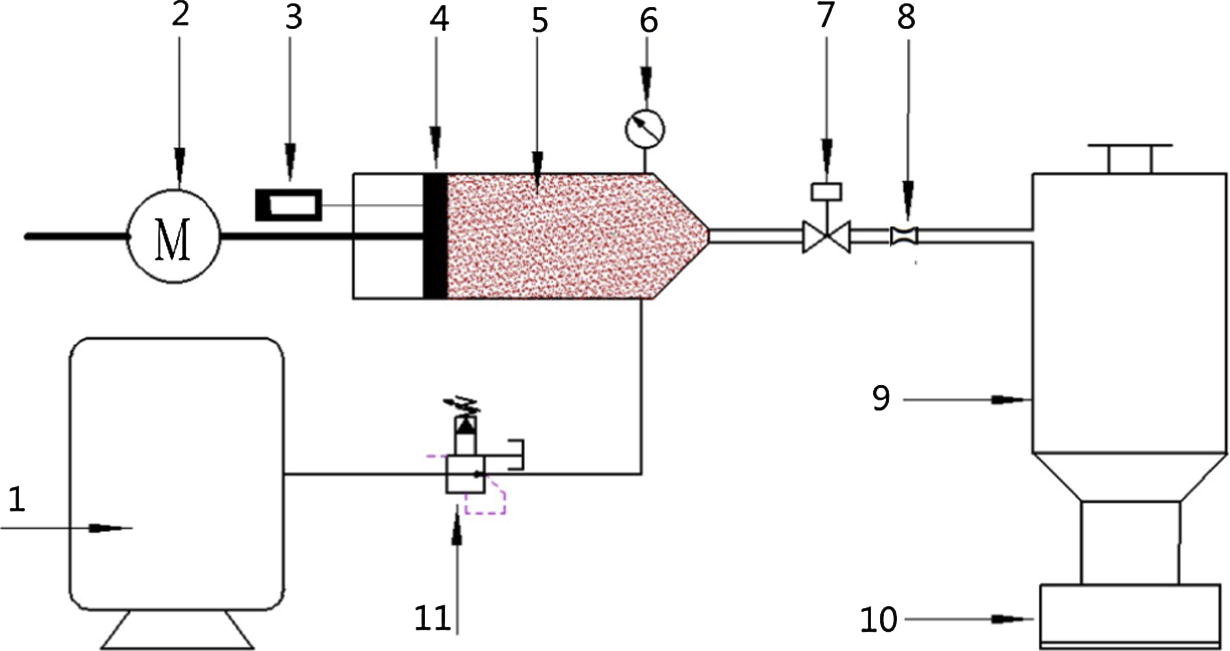
\includegraphics[width=\textwidth]{../report_assets/motor_driven.png}
        \caption*{Motor Driven Piston~\cite{SUN201630}}
    \end{minipage}
    \hfill
    \begin{minipage}{0.55\textwidth}
        \centering
        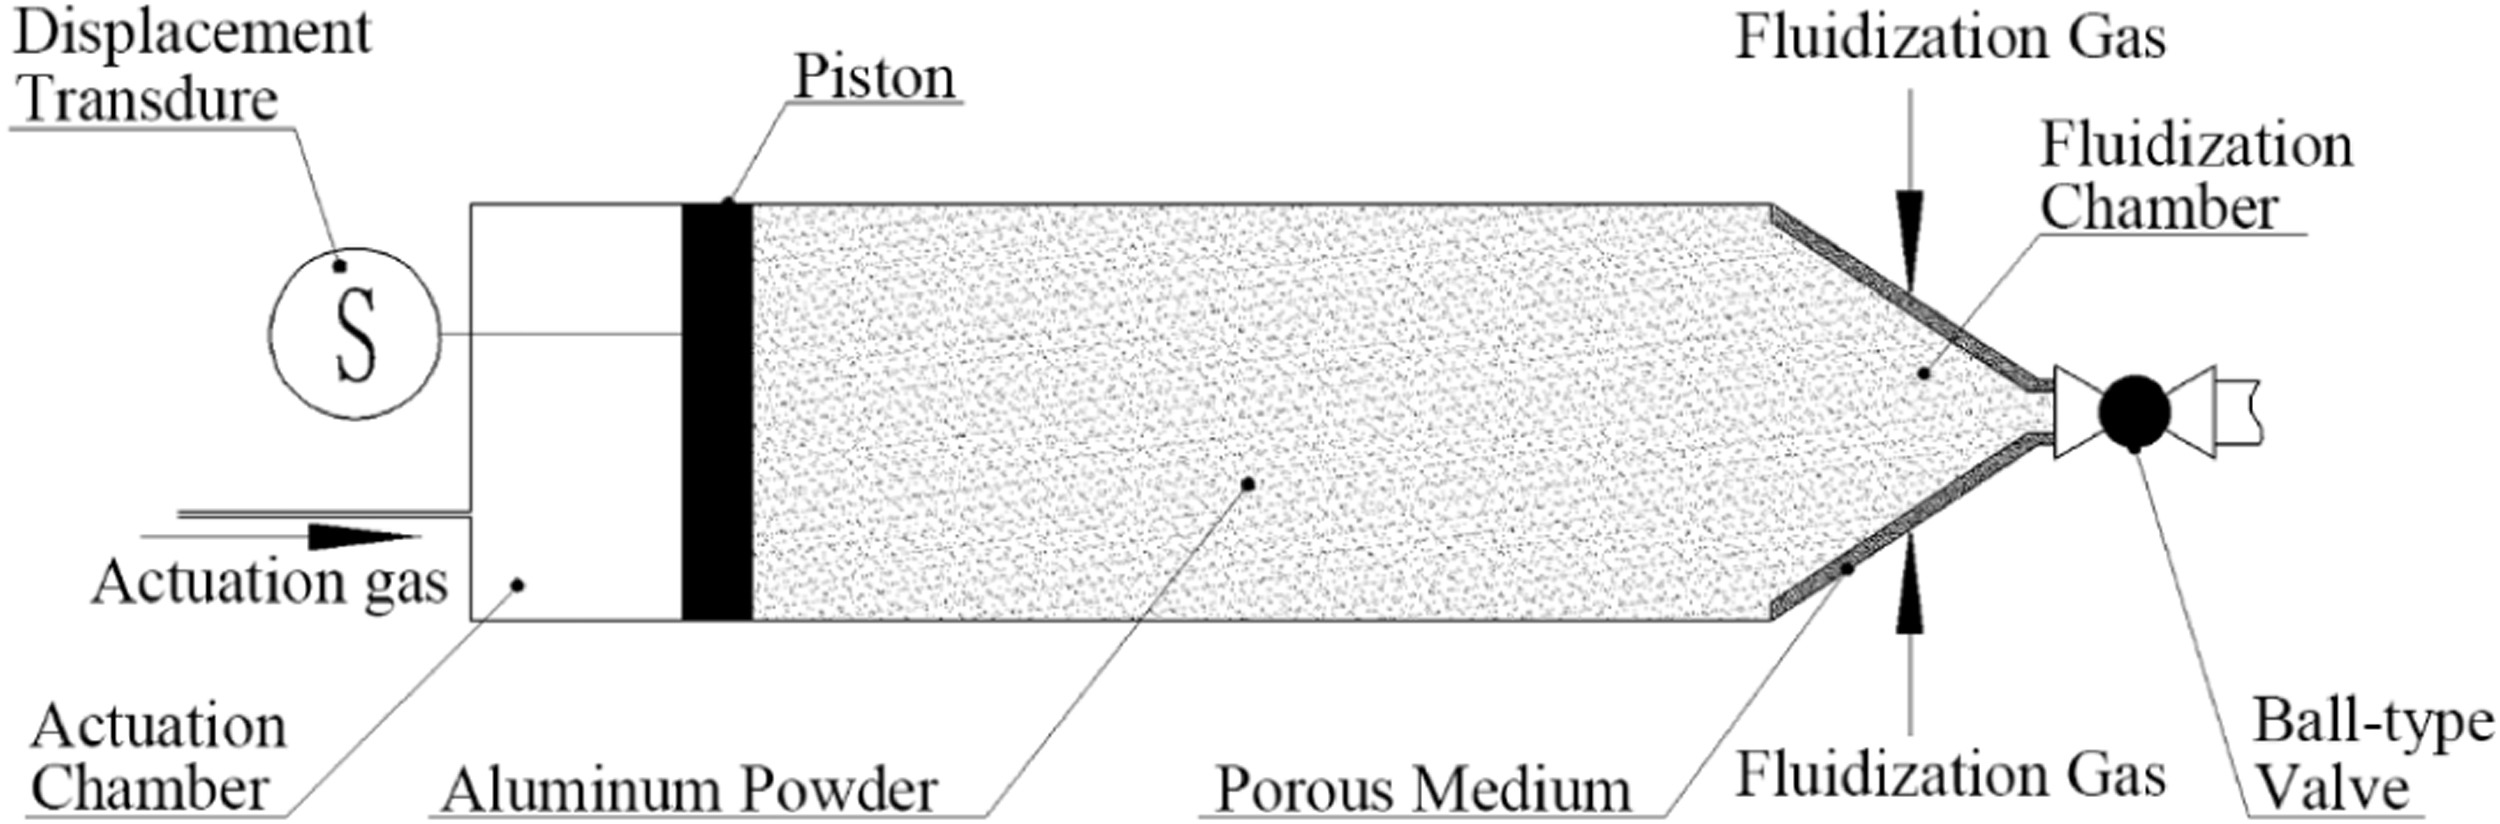
\includegraphics[width=\textwidth]{../report_assets/gas_driven.png}
        \caption*{Gas Driven Piston~\cite{Li2016}}
    \end{minipage}
    \caption{Examples of Gas and Motor Actuated Pistons from Literature}\label{fig:actuation-piston}
\end{figure}

The second innovation involved fluidising the powder from both the piston face and the end of the tank, as shown in \autoref{fig:fluid-from-the-back}. It has been demonstrated that fluidising further back in the tank results in higher mass flow rates and reduces the amount of powder left in the system~\cite{Tang22}. This means the feed systems fluidised at the inlet have a broader operating range of mass flow rates.
\begin{figure}[htbp]
    \centering
    
    \begin{minipage}{0.7\textwidth}
        \centering
        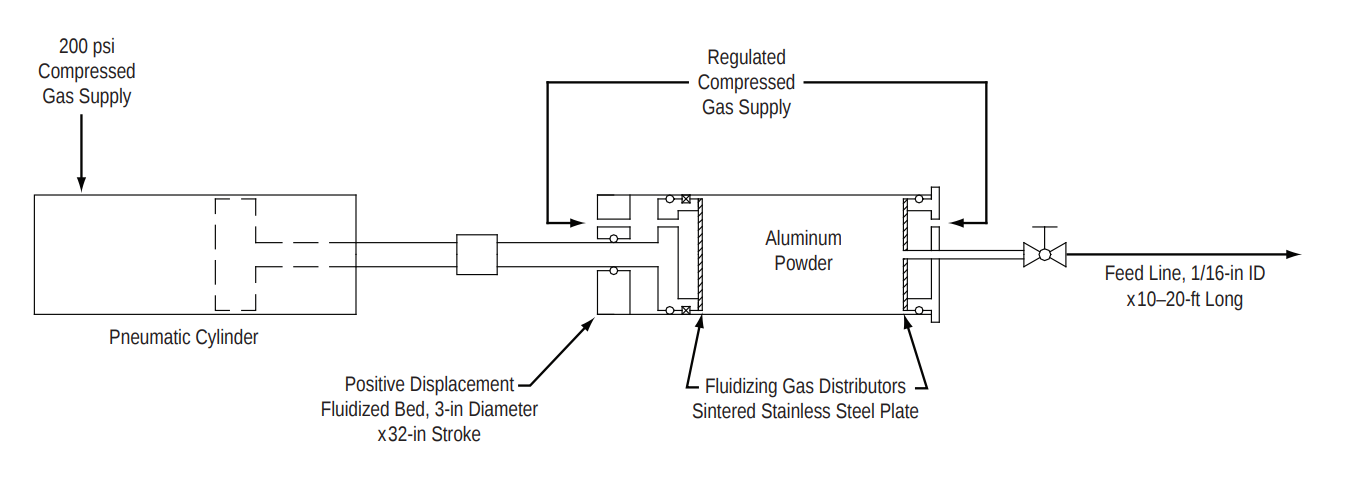
\includegraphics[width=\textwidth]{../report_assets/des_evo_3.png}
        \caption{Example of Fluidisation at the Inlet from Literature~\cite{NASA2008_20080002287}}\label{fig:fluid-from-the-back}
    \end{minipage}
   
\end{figure}

The final revision was removing the fluidisation at the end of the tank entirely, as seen in \autoref{fig:gas-permeable}. Designing the tank outlet to include a porous medium in its walls requires additional structural reinforcement, which increases the overall mass. Furthermore, the extra plumbing needed to supply fluidising gas to the outlet adds unnecessary mass, which can be avoided by fluidising solely from the rear.
\begin{figure}[htbp]
    \centering
    
    \begin{minipage}{0.6\textwidth}
        \centering
        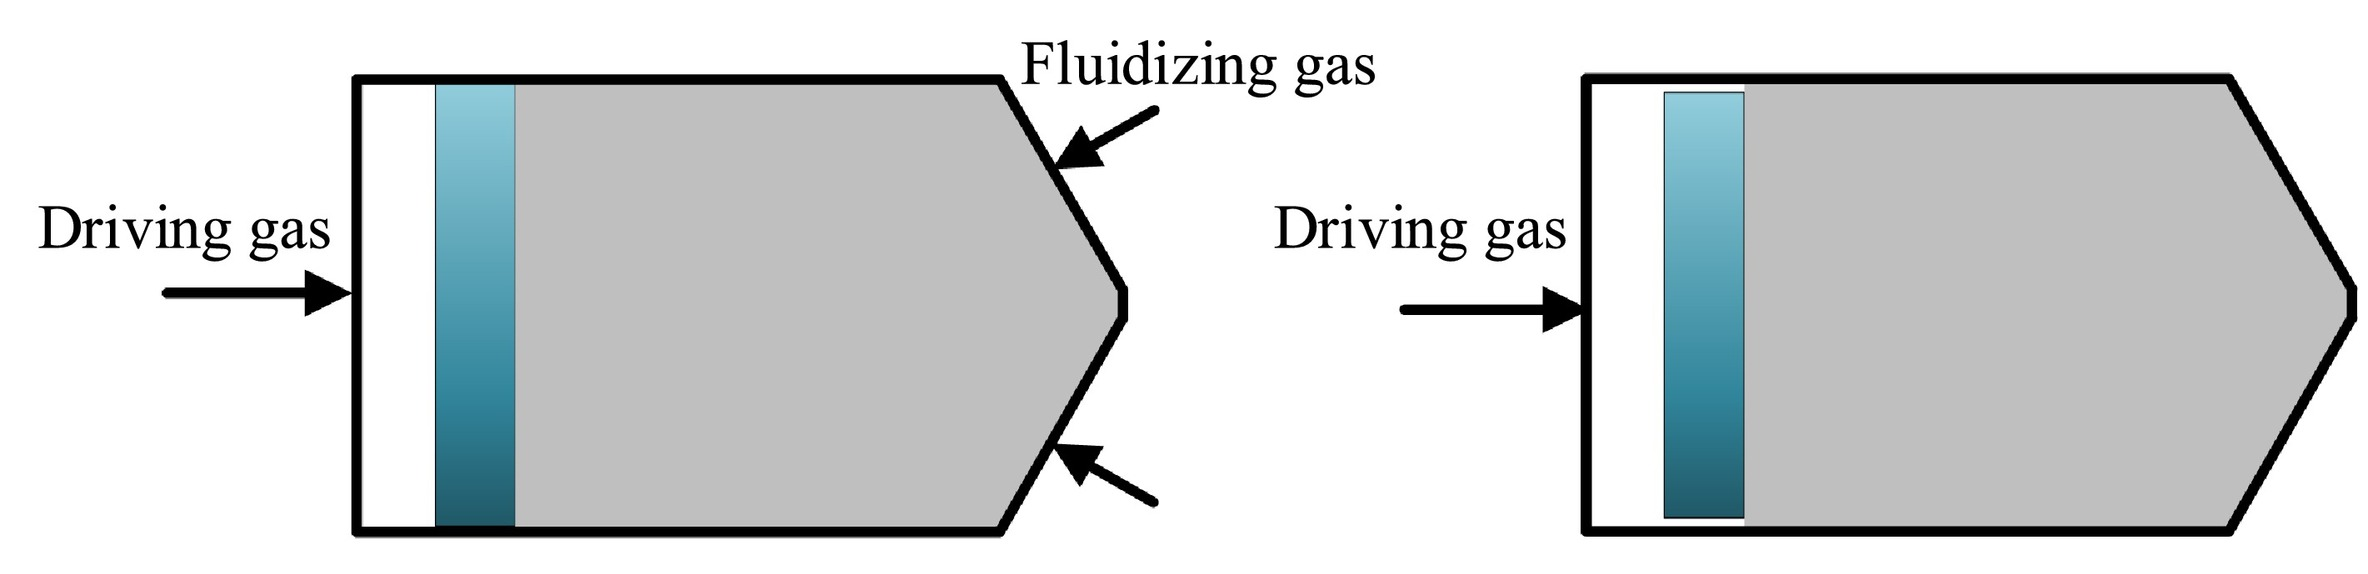
\includegraphics[width=\textwidth]{../report_assets/des_evo_1.png}
        \caption{Outlet Fluidised and Inlet Fluidised Designs~\cite{TANG2023118406}}\label{fig:gas-permeable}
    \end{minipage}
   
\end{figure}

Powder feed systems for powder-fed rocket motors have many similarities with CSAM feed systems but differ in one notable respect. While the particles in cold spray are fed into atmospheric conditions, or vacuum conditions for space applications, the particles in an engine are fed into the high-pressure combustion chamber. This means that the downstream pressure in the two systems differs significantly, which explains why the majority of the literature focuses on high-pressure powder feed systems. Given that lower pressures, $<1\,\mathrm{MPa}$, are less extensively investigated, this report contributes to the analysis of such conditions.
% A commonly cited first implementation of a fluisising powder feed system consists of a cylindrical tank with a piston to constrain the powder to the outlet~\cite{LI2021712}. As this paper is no longer in the public domain, the author assumes that the piston is motor actuated as the use of gas-actuated pistons is often credited to later work~\cite{TANG2023118406} and how the tank is fluidised is unknown. The gas actuated piston revisions pass the fluidising gas down the piston rod and through a gas-permeable piston face~\cite{Loftus1972}. Close to the outlet there is a porous section in which the fluidising gas is supplied. Despite the number of papers referencing this research, the author is unable to validate whether this is still in the public domain. This design was improved upon by pneumatically actuating the piston and supplying the fluidising gas through the piston shaft, with the gas exiting a porous plate mounted on the piston face~\cite{Loftus1972}. 

\section{Propellent Management Devices}
The need to store material in space is not new and has received extensive research attention, particularly in the context of propellant storage. Like the manufacturing system presented later, propulsion systems can be disturbed or damaged if the contents of the tank are not properly constrained to the outlet~\cite{Hartwig2016}. Solutions to this problem already exist in the form of propellant management devices.
\begin{figure}[htbp]
    \centering
    
    \begin{minipage}{0.25\textwidth}
        \centering
        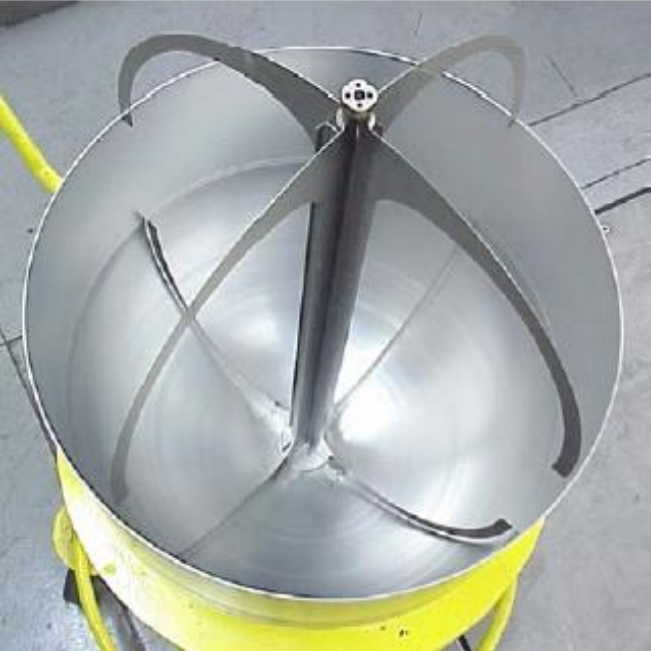
\includegraphics[width=\textwidth]{../report_assets/vane.png}
        \caption{Tank Vanes~\cite{Hartwig2016}}\label{fig:vane}
    \end{minipage}
    \hspace{3em}
    \begin{minipage}{0.47\textwidth}
        \centering
        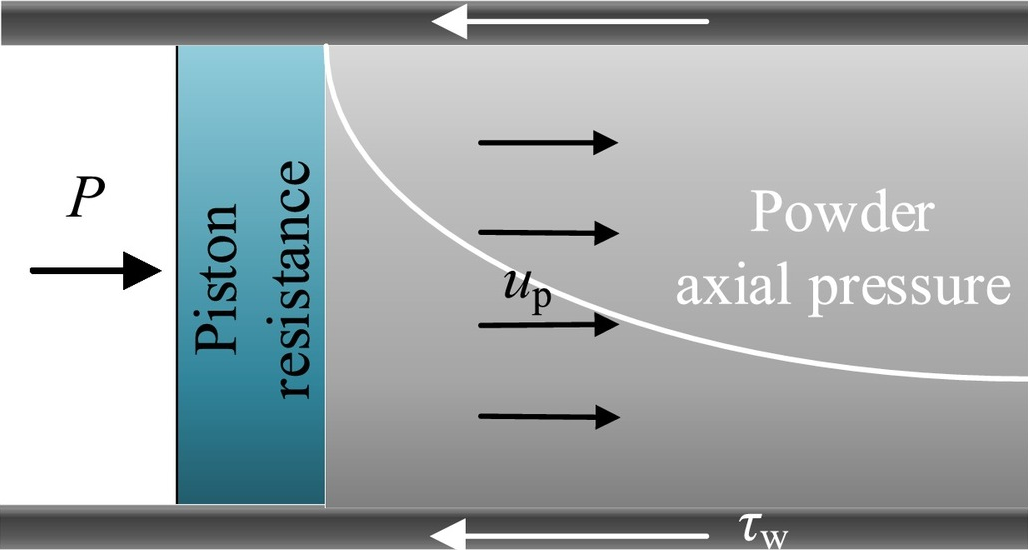
\includegraphics[width=\textwidth]{../report_assets/piston.png}
        \caption{Piston Tank Diagram~\cite{TANG2023118406}}\label{fig:piston}
    \end{minipage}
    
\end{figure}
Vanes, seen in \autoref{fig:vane}, sponges and galleries have been well tested in microgravity environments~\cite{Hartwig2016} but they rely on surface tension and are therefore only applicable to storing liquid. Positive expulsion devices such as bladders, diaphragms and pistons, seen in \autoref{fig:piston}, mechanically force propellant towards the outlet, and are thus suitable for powder applications. 

In addition to enabling more reliable powder dispensation, constraining the powder can prevent problematic dynamics such as sloshing from occuring within the tank. This reduces the system's footprint on the rest of the spacecraft and simplifies attitude control.


% sloshing phenomenon, surface tension doesnt work, piston tanks and common issues.
% 1
% A Detailed Historical Review of Propellant Management
% Devices for Low Gravity Propellant Acquisition
% in jan folder
% given extra time come back to this and try and cite stuff about surface tension and cite maybe the rate of usage
\section{Management of Bulk Powder}\label{sec:bulk-powder}
Powder in a tightly-packed (bulk) form exhibits entirely different dynamics from powder in a fluidised state and is more complex to describe. This complexity arises from the different types of interparticle forces~\cite{ZAFAR2017389}, the changing nature of contact points and friction due to plastic and elastic deformation~\cite{TALEBI2024211} and the limited freedom for particles to rearrange. 
\begin{figure}[htbp]
    \centering
    \begin{minipage}{0.6\textwidth}
        \centering
        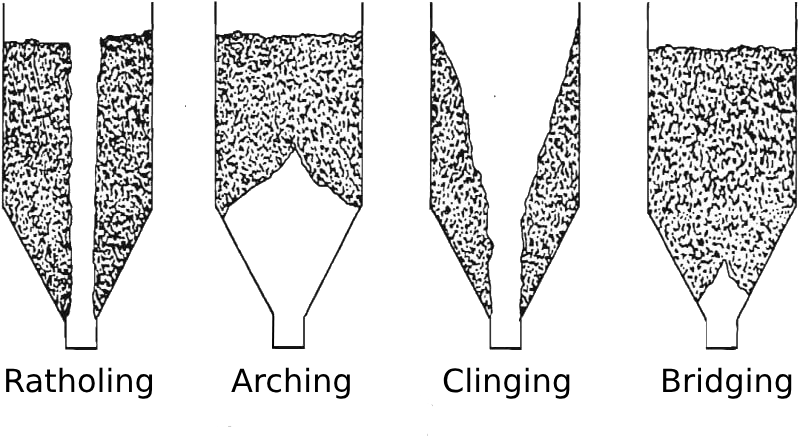
\includegraphics[width=\textwidth]{../report_assets/bridging.png}
        \caption{Common Powder Structures~\cite{911Metallurgist_binsflow}}\label{fig:bulk_powder_structures}
    \end{minipage}
\end{figure}
This means powders respond to stress in a manner intermediate between a fluid and a frictional solid: they dilate under shear, compact under normal load, and can sustain stable structures, such as those shown in \autoref{fig:bulk_powder_structures}, that block flow in hoppers. 
\section{Modelling Two-Phase flow}
Given the high cost of conducting experiments in microgravity, this project relies on correlating simulated behaviour under gravity with the experimental results, and then comparing this with the simulations conducted under microgravity conditions. Therefore, the simulation model used is outlined below.

Due to the wide variety of two-phase flow types, there are numerous ways to model the behaviour.  The general idea applies the conservation of mass, momentum and energy equations for both phases over a fixed control volume. While this formulation is sufficient for performing direct numerical simulation, simplifying assumptions are often made to avoid the unrealistic computational demands~\cite{enwald1996eulerian}. 

Fluidising beds are typically simulated using one of two main approaches: the Eulerian-Lagrangian method or the Eulerian-Eulerian method~\cite{C6RA28615A}. The Eulerian-Lagrangian treats the particles as a discrete phase and the fluidising gas as a continuum. It tracks the dynamics of individual particles in a Lagrangian reference frame and couples them to the gas through interphase momentum exchange~\cite{SUBRAMANIAM2013215}. The Eulerian-Eulerian method models both phases as interpenetrating continua, tracking the local volume fraction of the particle phase and using constitutive equations from granular flow theory to couple the two~\cite{C6RA28615A}. As discussed in \autoref{sec:numerical-setup}, the Eulerian-Eulerian model is most applicable to the system under study and is therefore outlined further.

While the drag model is not a constitutive equation in the strict sense, it functions as one in Eulerian-Eulerian models by closing the system of equations. Therefore the choice of drag model significant impacts the resulting dynamics, particularly with respect to the behaviour of bubbles and bed expansion. The Gidaspow model has found to be the most representative for fluidised beds~\cite{C6RA28615A}.

